\section{Experimento BRDF Minnaert}
\label{section-experiment-minnaert}

Este experimento foi realizado seguindo os princípios do artigo de Minnaert \cite{minnaert1941reciprocity}. Nele, é apresentado um modelo de reflexão que introduz um método para descrever superfícies que exibem comportamentos encontrados em superfícies porosas, como a lua. As equações desse experimento estão na \autoref{fig-minnaert-eqlang-latex}. O código-fonte pode ser encontrado no \autoref{cod-minnaert-eqlang}. O GLSL gerado pode ser encontrado no \autoref{cod-minnaert-glsl-pt-1} e no \autoref{cod-minnaert-glsl-pt-2}, enquanto os resultados de renderização podem ser observados na \autoref{fig-minnaert-eqlang} e os \textit{plots} na \autoref{fig-minnaert-plots}.


%%%%%%%%%%%%%%%%%%%%%%%%%%%%%%%%%%%%%%%%%%%%%%%%%
\subsection{Representação em documento \LaTeX{}}
%%%%%%%%%%%%%%%%%%%%%%%%%%%%%%%%%%%%%%%%%%%%%%%%%
\begin{figure}[H]
    \caption{\label{fig-minnaert-eqlang-latex} \small Equações da BRDF do experimento Minnaert em documento \LaTeX{}.}
    \begin{center}
        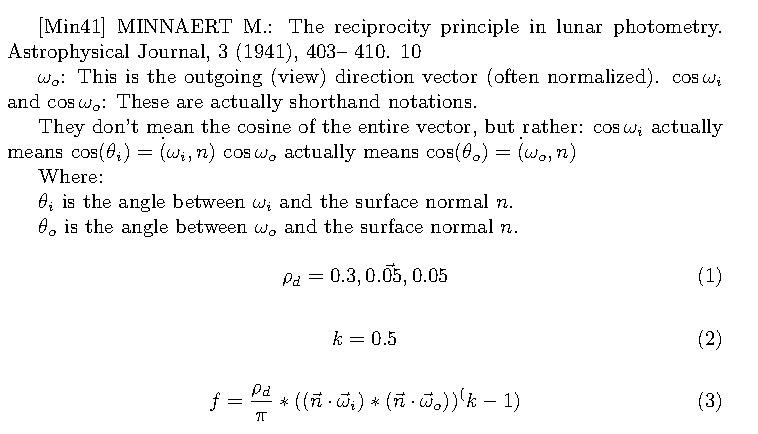
\includegraphics[scale=0.92]{./Imagens/brdfs/minnaert.pdf}
    \end{center}
\end{figure}

%%%%%%%%%%%%%%%%%%%%%%%%%%%%%%%%%%%%%%%%%%%%%%%%%
\subsection{Código Fonte em \texttt{EquationLang}}
%%%%%%%%%%%%%%%%%%%%%%%%%%%%%%%%%%%%%%%%%%%%%%%%%
\begin{codigo}[H]
    \caption{\small Código fonte da BRDF do experimento Minnaert.}
    \label{cod-minnaert-eqlang}
\begin{lstlisting}[language=tex, frame=none, inputencoding=utf8]
[Min41] MINNAERT M.: The reciprocity principle in lunar photometry. Astrophysical Journal, 3 (1941), 403- 410. 10

$\omega_o$: This is the outgoing (view) direction vector (often normalized).
$\cos\omega_i$ and $\cos\omega_o$: These are actually shorthand notations.

They don't mean the cosine of the entire vector, but rather:
$\cos\omega_i$ actually means $\cos(\theta_i) = \dot(\omega_i, n)$
$\cos\omega_o$ actually means $\cos(\theta_o) = \dot(\omega_o, n)$

Where:

$\theta_i$ is the angle between $\omega_i$ and the surface normal $n$.

$\theta_o$ is the angle between $\omega_o$ and the surface normal $n$.

\begin{equation}
    \rho_{d} = \vec{0.3,0.05,0.05}
\end{equation}

\begin{equation}
k = 0.5
\end{equation}

\begin{equation}
f = \frac{\rho_{d}}{\pi} * ((\vec{n} \cdot \vec \omega_i)*(\vec{n} \cdot \vec \omega_o))^{(k-1)}
\end{equation}
\end{lstlisting}
\end{codigo}

%%%%%%%%%%%%%%%%%%%%%%%%%%%%%%%%%%%%%%%%%%%%%%%%%
\subsection{Código GLSL Gerado}
%%%%%%%%%%%%%%%%%%%%%%%%%%%%%%%%%%%%%%%%%%%%%%%%%
\begin{codigo}[H]
    \caption{\small Saída do compilador: código GLSL da BRDF do experimento Minnaert (parte 1 de 2).}
    \label{cod-minnaert-glsl-pt-1}
\begin{lstlisting}[language=C, inputencoding=utf8]
analytic ::begin parameters
#[type][name][min val][max val][default val]
::end parameters
::begin shader
//////////// START OF BUILTINS DECLARTION ////////////
vec3 var_0_vec_h;
vec3 var_3_vec_n;
float var_10_theta_h;
float var_11_theta_d;
float var_1_pi;
float var_2_epsilon;
vec3 var_4_vec_omega_i;
float var_5_theta_i;
float var_6_phi_i;
vec3 var_7_vec_omega_o;
float var_8_theta_o;
float var_9_phi_o;
//////////// END OF BUILTINS DECLARTION ////////////

//////////// START OF USER DECLARED ////////////
vec3 var_12_rho_d;
float var_13_k;
vec3 var_14_f;
//////////// END OF USER DECLARED ////////////

//////////// START FUNCTIONS DECLARATIONS ////////////
//////////// END FUNCTIONS DECLARATIONS ////////////
\end{lstlisting}
\end{codigo}

\begin{codigo}[H]
    \caption{\small Saída do compilador: código GLSL da BRDF do experimento Minnaert (parte 2 de 2).}
    \label{cod-minnaert-glsl-pt-2}
\begin{lstlisting}[language=C, inputencoding=utf8]
vec3 BRDF(vec3 L, vec3 V, vec3 N, vec3 X, vec3 Y) {

  //////////// START OF BUILTINS INITIALIZATION ////////////
  var_0_vec_h = normalize(L + V);
  var_3_vec_n = normalize(N);
  var_1_pi = 3.141592653589793;
  var_2_epsilon = 1.192092896e-07;
  var_4_vec_omega_i = L;
  var_5_theta_i = atan(var_4_vec_omega_i.y, var_4_vec_omega_i.x);
  var_6_phi_i = atan(sqrt(var_4_vec_omega_i.y * var_4_vec_omega_i.y +
                          var_4_vec_omega_i.x * var_4_vec_omega_i.x),
                     var_4_vec_omega_i.z);
  var_7_vec_omega_o = V;
  var_8_theta_o = atan(var_7_vec_omega_o.y, var_7_vec_omega_o.x);
  var_9_phi_o = atan(sqrt(var_7_vec_omega_o.y * var_7_vec_omega_o.y +
                          var_7_vec_omega_o.x * var_7_vec_omega_o.x),
                     var_7_vec_omega_o.z);
  var_10_theta_h = acos(dot(var_0_vec_h, N));
  var_11_theta_d = acos(dot(var_0_vec_h, var_4_vec_omega_i));
  //////////// END OF BUILTINS INITIALIZATION ////////////

  var_12_rho_d = vec3(0.3, 0.05, 0.05);
  var_13_k = 0.5;
  var_14_f = ((var_12_rho_d / var_1_pi) *
              pow((((dot(var_3_vec_n, var_4_vec_omega_i)) *
                    (dot(var_3_vec_n, var_7_vec_omega_o)))),
                  ((var_13_k - 1.0))));

  return vec3(var_14_f);
}
\end{lstlisting}
\end{codigo}
%%%%%%%%%%%%%%%%%%%%%%%%%%%%%%%%%%%%%%%%%%%%%%%%%
\subsection{Visualização do Resultado}
%%%%%%%%%%%%%%%%%%%%%%%%%%%%%%%%%%%%%%%%%%%%%%%%%
\begin{figure}[H]
    \caption{\small{\textit{Plots} da distribuição de reflexão especular e difusa do experimento Minnaert.}}
    \label{fig-minnaert-plots}
\minipage{0.48\textwidth}
    \vspace{42px}
  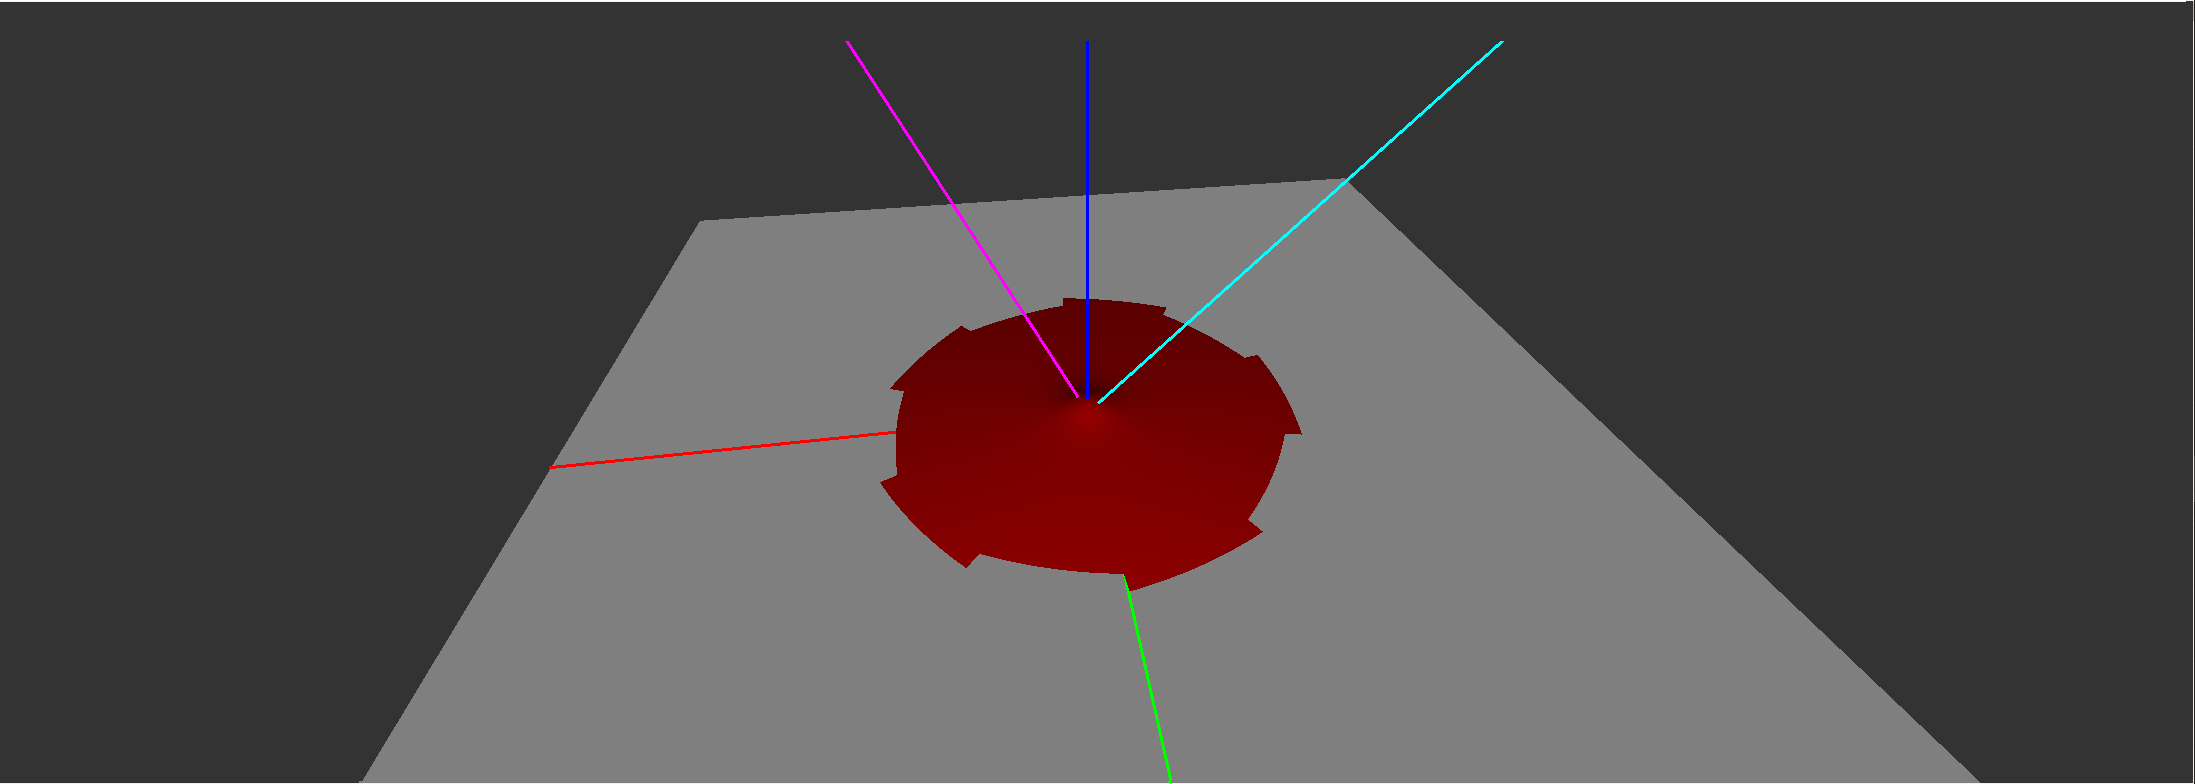
\includegraphics[width=\linewidth]{./Imagens/brdfs/minnaert-3D-plot}
    % \vspace{0.1px}
    \legend{ \small (a) 3D \textit{plot}}
\endminipage\hfill
\minipage{0.48\textwidth}
  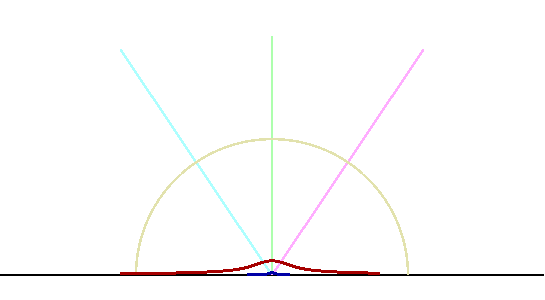
\includegraphics[width=\linewidth]{./Imagens/brdfs/minnaert-polar-plot.png}
    \legend{ \small (b) \textit{Polar plot}}
\endminipage\hfill
\end{figure}

\begin{figure}[H]
    \caption{\small{Objetos 3D renderizados pelo experimento Minnaert.}}\label{fig-minnaert-eqlang}
\minipage{0.32\textwidth}
  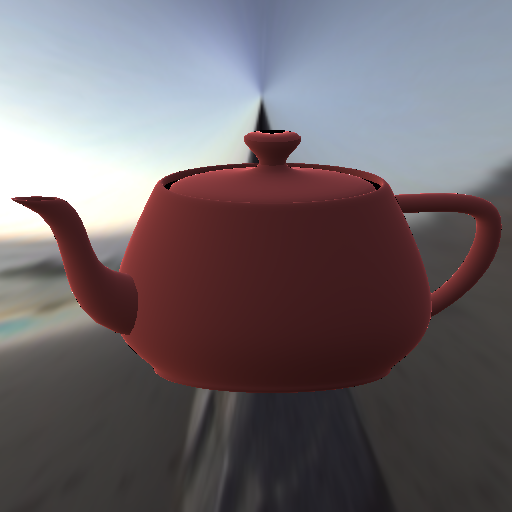
\includegraphics[width=\linewidth]{./Imagens/brdfs/minnaert-teapot.png}
    \legend{ \small (a) \textit{Teapot}}
\endminipage\hfill
\minipage{0.32\textwidth}
  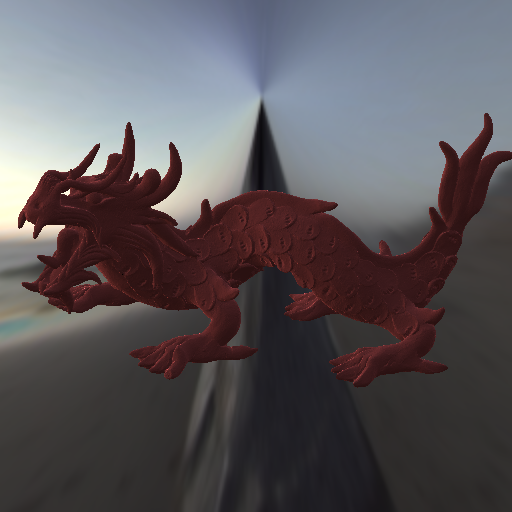
\includegraphics[width=\linewidth]{./Imagens/brdfs/minnaert-dragon.png}
    \legend{ \small (b) Dragão de Stanford}
\endminipage\hfill
\minipage{0.32\textwidth}%
  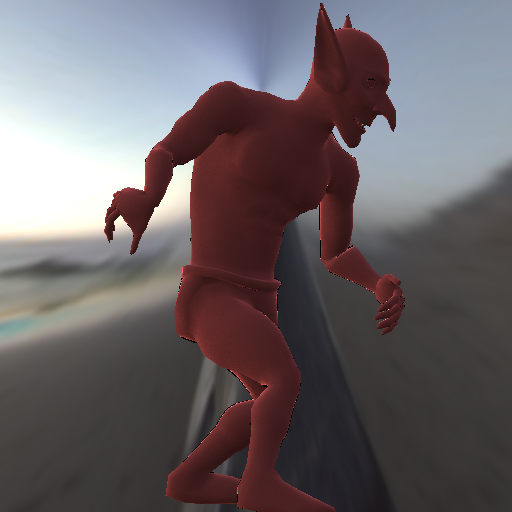
\includegraphics[width=\linewidth]{./Imagens/brdfs/minnaert-goblin.png}
    \legend{ \small (c) Goblin}
\endminipage
\end{figure}

